\documentclass[tikz,border=10pt]{standalone}
\usetikzlibrary{calc}
\begin{document}
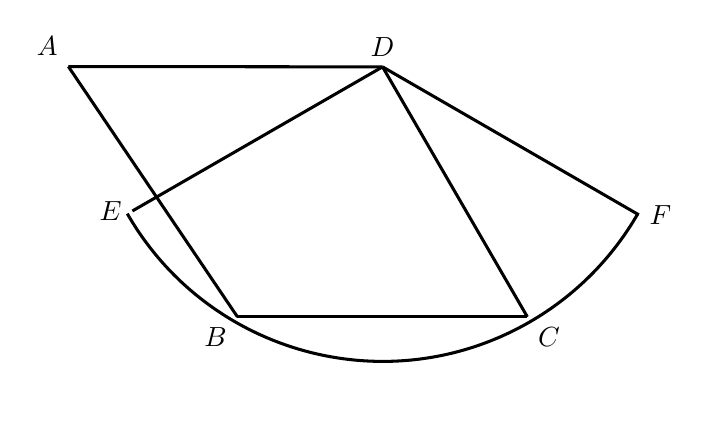
\begin{tikzpicture}[line join=round, line width=1.1pt,
  every label/.style={font=\fontsize{10.5}{12.6}\selectfont}]
\coordinate (A) at (-3.599,1.856);
\coordinate (B) at (-1.452,-1.323);
\coordinate (C) at (2.230,-1.323);
\coordinate (D) at (0.391,1.852);
\coordinate (F) at (3.645,-0.027);



\coordinate (E) at (-2.786,0.022);


\draw (A) -- (D);
\draw (A) -- (B);
\draw (B) -- (C);
\draw (C) -- (D);
\draw (D) -- (E);
\draw (D) -- (F);


\draw ($(D)+(209.900:3.740)$) arc[start angle=209.900, end angle=330.000, radius=3.740];


\node[above left] at (A) {$A$};
\node[above] at (D) {$D$};
\node[below left] at (B) {$B$};
\node[below right] at (C) {$C$};
\node[left] at (E) {$E$};
\node[right] at (F) {$F$};
\end{tikzpicture}
\end{document}